\hypertarget{vectornav_8h}{}\section{src/hammerhead/hardware\+\_\+stack/vectornav/include/vectornav/vectornav.h File Reference}
\label{vectornav_8h}\index{src/hammerhead/hardware\+\_\+stack/vectornav/include/vectornav/vectornav.\+h@{src/hammerhead/hardware\+\_\+stack/vectornav/include/vectornav/vectornav.\+h}}
{\ttfamily \#include \char`\"{}vn100.\+h\char`\"{}}\\*
{\ttfamily \#include \char`\"{}vn200.\+h\char`\"{}}\\*
{\ttfamily \#include \char`\"{}vn\+\_\+math.\+h\char`\"{}}\\*
Include dependency graph for vectornav.\+h\+:
\nopagebreak
\begin{figure}[H]
\begin{center}
\leavevmode
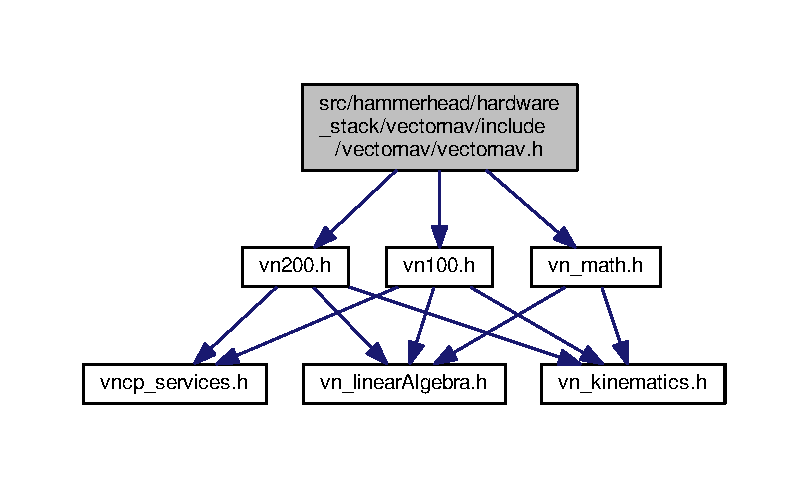
\includegraphics[width=350pt]{vectornav_8h__incl}
\end{center}
\end{figure}
This graph shows which files directly or indirectly include this file\+:
\nopagebreak
\begin{figure}[H]
\begin{center}
\leavevmode
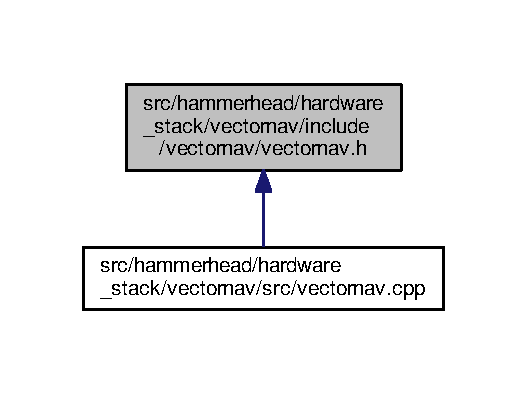
\includegraphics[width=253pt]{vectornav_8h__dep__incl}
\end{center}
\end{figure}


\subsection{Detailed Description}
\hypertarget{index_LICENSE}{}\subsection{L\+I\+C\+E\+N\+SE}\label{index_LICENSE}
M\+IT License (M\+IT)

Copyright (c) 2012 Vector\+Nav Technologies, L\+LC

Permission is hereby granted, free of charge, to any person obtaining a copy of this software and associated documentation files (the \char`\"{}\+Software\char`\"{}), to deal in the Software without restriction, including without limitation the rights to use, copy, modify, merge, publish, distribute, sublicense, and/or sell copies of the Software, and to permit persons to whom the Software is furnished to do so, subject to the following conditions\+:

The above copyright notice and this permission notice shall be included in all copies or substantial portions of the Software.

T\+HE S\+O\+F\+T\+W\+A\+RE IS P\+R\+O\+V\+I\+D\+ED \char`\"{}\+A\+S I\+S\char`\"{}, W\+I\+T\+H\+O\+UT W\+A\+R\+R\+A\+N\+TY OF A\+NY K\+I\+ND, E\+X\+P\+R\+E\+SS OR I\+M\+P\+L\+I\+ED, I\+N\+C\+L\+U\+D\+I\+NG B\+UT N\+OT L\+I\+M\+I\+T\+ED TO T\+HE W\+A\+R\+R\+A\+N\+T\+I\+ES OF M\+E\+R\+C\+H\+A\+N\+T\+A\+B\+I\+L\+I\+TY, F\+I\+T\+N\+E\+SS F\+OR A P\+A\+R\+T\+I\+C\+U\+L\+AR P\+U\+R\+P\+O\+SE A\+ND N\+O\+N\+I\+N\+F\+R\+I\+N\+G\+E\+M\+E\+NT. IN NO E\+V\+E\+NT S\+H\+A\+LL T\+HE A\+U\+T\+H\+O\+RS OR C\+O\+P\+Y\+R\+I\+G\+HT H\+O\+L\+D\+E\+RS BE L\+I\+A\+B\+LE F\+OR A\+NY C\+L\+A\+IM, D\+A\+M\+A\+G\+ES OR O\+T\+H\+ER L\+I\+A\+B\+I\+L\+I\+TY, W\+H\+E\+T\+H\+ER IN AN A\+C\+T\+I\+ON OF C\+O\+N\+T\+R\+A\+CT, T\+O\+RT OR O\+T\+H\+E\+R\+W\+I\+SE, A\+R\+I\+S\+I\+NG F\+R\+OM, O\+UT OF OR IN C\+O\+N\+N\+E\+C\+T\+I\+ON W\+I\+TH T\+HE S\+O\+F\+T\+W\+A\+RE OR T\+HE U\+SE OR O\+T\+H\+ER D\+E\+A\+L\+I\+N\+GS IN T\+HE S\+O\+F\+T\+W\+A\+RE.\hypertarget{vn__math_8h_DESCRIPTION}{}\subsection{D\+E\+S\+C\+R\+I\+P\+T\+I\+ON}\label{vn__math_8h_DESCRIPTION}
This header file includes all of the header file inclusions needed to use all of the features of the Vector\+Nav C/\+C++ Library.\hypertarget{vectornav_8h_VectorNav}{}\subsection{C/\+C++ Library}\label{vectornav_8h_VectorNav}
The Vector\+Nav C/\+C++ Library allows interfacing with Vector\+Nav\textquotesingle{}s orientation and inertial sensor products.\hypertarget{vectornav_8h_Samples}{}\subsection{Samples}\label{vectornav_8h_Samples}
The folder {\itshape samples} contains sample projects that can be immediately compiled in various environments. The following sections walk through compiling and running the samples provided.\hypertarget{vectornav_8h_vn100LinuxSample}{}\subsubsection{Linux Sample (\+V\+N-\/100)}\label{vectornav_8h_vn100LinuxSample}
This samples illustrates how to setup an environment for compiling the Vector\+Nav C/\+C++ Library for use with a V\+N-\/100 device.


\begin{DoxyEnumerate}
\item Open the file {\ttfamily main.\+c} and change the configuration defines at the top to your environment specifics.
\begin{DoxyItemize}
\item For the C\+O\+M\+\_\+\+P\+O\+RT define, normal physical C\+OM ports typically will be in the form of {\ttfamily /dev/tty\+S1}. If you are using an F\+T\+DI U\+S\+B-\/to-\/\+Serial chip (typically found on U\+SB cables supplied with V\+N-\/100 Rugged Kits or on a V\+N-\/100 Development Board), the necessary drivers are already include in kernel version 2.\+6.\+31 and later and can be accessed in the form of {\ttfamily /dev/tty\+U\+S\+B0}.
\item For the B\+A\+U\+D\+\_\+\+R\+A\+TE define, change it to the currently saved baudrate speed of your Vector\+Nav device.
\end{DoxyItemize}
\item From a terminal window, browse to the folder {\itshape samples/vn100\+\_\+linux} and compile by typing the command {\ttfamily make}.
\item The sample program may then be run by executing the command {\ttfamily ./main} .
\begin{DoxyItemize}
\item Some Linux flavors may require administrative access to the C\+OM port. If you receive an error message indicating invalid access privileges, try exeucting the command as {\ttfamily sudo ./main} .
\end{DoxyItemize}
\end{DoxyEnumerate}\hypertarget{vectornav_8h_vn200LinuxSample}{}\subsubsection{Linux Sample (\+V\+N-\/200)}\label{vectornav_8h_vn200LinuxSample}
This samples illustrates how to setup an environment for compiling the Vector\+Nav C/\+C++ Library for use with a V\+N-\/200 device.


\begin{DoxyEnumerate}
\item Open the file {\ttfamily main.\+c} and change the configuration defines at the top to your environment specifics.
\begin{DoxyItemize}
\item For the C\+O\+M\+\_\+\+P\+O\+RT define, normal physical C\+OM ports typically will be in the form of {\ttfamily /dev/tty\+S1}. If you are using an F\+T\+DI U\+S\+B-\/to-\/\+Serial chip (typically found on U\+SB cables supplied with V\+N-\/200 Rugged Kits or on a V\+N-\/200 Development Board), the necessary drivers are already include in kernel version 2.\+6.\+31 and later and can be accessed in the form of {\ttfamily /dev/tty\+U\+S\+B0}.
\item For the B\+A\+U\+D\+\_\+\+R\+A\+TE define, change it to the currently saved baudrate speed of your Vector\+Nav device.
\end{DoxyItemize}
\item From a terminal window, browse to the folder {\itshape samples/vn200\+\_\+linux} and compile by typing the command {\ttfamily make}.
\item The sample program may then be run by executing the command {\ttfamily ./main} .
\begin{DoxyItemize}
\item Some Linux flavors may require administrative access to the C\+OM port. If you receive an error message indicating invalid access privileges, try exeucting the command as {\ttfamily sudo ./main} .
\end{DoxyItemize}
\end{DoxyEnumerate}\hypertarget{vectornav_8h_includingInExistingProject}{}\subsection{Including in Existing Projects}\label{vectornav_8h_includingInExistingProject}
The following sections provide guidance for using the library in your project.\hypertarget{vectornav_8h_microsoftVisualStudioVn100Usage}{}\subsubsection{Microsoft Visual Studio (\+V\+N-\/100)}\label{vectornav_8h_microsoftVisualStudioVn100Usage}
The following steps will walk you through including the Vector\+Nav C/\+C++ Library into your existing C or C++ project to access a V\+N-\/100 device. You can also find an example usage of the library at \hyperlink{vn100_windows_basic_8c-example}{vn100\+\_\+windows\+\_\+basic.c}.


\begin{DoxyEnumerate}
\item Add the code files \hyperlink{vn100_8c}{src/vn100.\+c} and src/arch/win32/vncp\+\_\+services.\+c to your project.
\begin{DoxyItemize}
\item Right-\/click on your project file and select {\itshape Add -\/$>$ Existing Item...} and browse to where you extracted the library files and select the two file.
\end{DoxyItemize}
\item Add an additional include directory to the libraries {\ttfamily include} folder.
\begin{DoxyItemize}
\item Right-\/click on your project file and select Properties. On the property pages, browse to {\itshape Configuration Properties -\/$>$ C/\+C++ -\/$>$ General}. For the property field {\itshape Additional Include Directories}, add a link to the library\textquotesingle{}s {\ttfamily include} folder.
\end{DoxyItemize}
\item Disable usage of precompiled headers for your project.
\begin{DoxyItemize}
\item Right-\/click on your project file and select Properties. Browse to the section {\itshape Configuration Properties -\/$>$ C/\+C++ -\/$>$ Precompiled Header} and select the option {\itshape Not Using Precompiled Headers}.
\end{DoxyItemize}
\item Add the include line {\ttfamily \#include \char`\"{}vectornav.\+h\char`\"{}} to the top of your code file to get access to all of the types and functions provided by the library.
\end{DoxyEnumerate}\hypertarget{vectornav_8h_microsoftVisualStudioVn200Usage}{}\subsubsection{Microsoft Visual Studio (\+V\+N-\/200)}\label{vectornav_8h_microsoftVisualStudioVn200Usage}
The following steps will walk you through including the Vector\+Nav C/\+C++ Library into your existing C or C++ project to access a V\+N-\/200 device. You can also find an example usage of the library at \hyperlink{vn200_windows_basic_8c-example}{vn200\+\_\+windows\+\_\+basic.c}.


\begin{DoxyEnumerate}
\item Add the code files src/vn200.\+c and src/arch/win32/vncp\+\_\+services.\+c to your project.
\begin{DoxyItemize}
\item Right-\/click on your project file and select {\itshape Add -\/$>$ Existing Item...} and browse to where you extracted the library files and select the two file.
\end{DoxyItemize}
\item Add an additional include directory to the libraries {\ttfamily include} folder.
\begin{DoxyItemize}
\item Right-\/click on your project file and select Properties. On the property pages, browse to {\itshape Configuration Properties -\/$>$ C/\+C++ -\/$>$ General}. For the property field {\itshape Additional Include Directories}, add a link to the library\textquotesingle{}s {\ttfamily include} folder.
\end{DoxyItemize}
\item Disable usage of precompiled headers for your project.
\begin{DoxyItemize}
\item Right-\/click on your project file and select Properties. Browse to the section {\itshape Configuration Properties -\/$>$ C/\+C++ -\/$>$ Precompiled Header} and select the option {\itshape Not Using Precompiled Headers}.
\end{DoxyItemize}
\item Add the include line {\ttfamily \#include \char`\"{}vectornav.\+h\char`\"{}} to the top of your code file to get access to all of the types and functions provided by the library.
\end{DoxyEnumerate}\hypertarget{vectornav_8h_linuxVn100Usage}{}\subsubsection{Linux (\+V\+N-\/100)}\label{vectornav_8h_linuxVn100Usage}
The following steps will walk you through adding the Vector\+Nav C/\+C++ Library to your Linux project to access a V\+N-\/100 device. You can also find an example usage of the library at \hyperlink{vn100_linux_basic_8c-example}{vn100\+\_\+linux\+\_\+basic.c}.


\begin{DoxyEnumerate}
\item Add lines to your makefile to compile the code files \hyperlink{vn100_8c}{src/vn100.\+c} and src/arch/linux/vncp\+\_\+services.\+c.
\begin{DoxyItemize}
\item Example lines...
\begin{DoxyItemize}
\item {\ttfamily gcc -\/c -\/\+Iinclude \hyperlink{vn100_8c}{src/vn100.\+c}}
\item {\ttfamily gcc -\/c -\/\+Iinclude src/arch/linux/vncp\+\_\+services.\+c}
\end{DoxyItemize}
\end{DoxyItemize}
\item When you link the all of the compiled files together, you will need to add a reference to the pthread library as well as the output object files from the previous step.
\begin{DoxyItemize}
\item Example linker command\+: {\ttfamily gcc -\/lpthread main.\+o vn100.\+o vncp\+\_\+services.\+o -\/o main}
\end{DoxyItemize}
\item In code files where you wish to access the functionality of the library, add the line {\ttfamily \#include \char`\"{}vectornav.\+h\char`\"{}} at the top of the code file. You will also need to add a reference to the include directory when you compile your code file.
\end{DoxyEnumerate}\hypertarget{vectornav_8h_linuxVn200Usage}{}\subsubsection{Linux (\+V\+N-\/200)}\label{vectornav_8h_linuxVn200Usage}
The following steps will walk you through adding the Vector\+Nav C/\+C++ Library to your Linux project to access a V\+N-\/200 device. You can also find an example usage of the library at \hyperlink{vn200_linux_basic_8c-example}{vn200\+\_\+linux\+\_\+basic.c}.


\begin{DoxyEnumerate}
\item Add lines to your makefile to compile the code files src/vn200.\+c and src/arch/linux/vncp\+\_\+services.\+c.
\begin{DoxyItemize}
\item Example lines...
\begin{DoxyItemize}
\item {\ttfamily gcc -\/c -\/\+Iinclude src/vn200.\+c}
\item {\ttfamily gcc -\/c -\/\+Iinclude src/arch/linux/vncp\+\_\+services.\+c}
\end{DoxyItemize}
\end{DoxyItemize}
\item When you link the all of the compiled files together, you will need to add a reference to the pthread library as well as the output object files from the previous step.
\begin{DoxyItemize}
\item Example linker command\+: {\ttfamily gcc -\/lpthread main.\+o vn200.\+o vncp\+\_\+services.\+o -\/o main}
\end{DoxyItemize}
\item In code files where you wish to access the functionality of the library, add the line {\ttfamily \#include \char`\"{}vectornav.\+h\char`\"{}} at the top of the code file. You will also need to add a reference to the include directory when you compile your code file. 
\end{DoxyEnumerate}